\documentclass[a4paper,14pt]{extarticle}

\usepackage[utf8x]{inputenc}
\usepackage[T1,T2A]{fontenc}
\usepackage[russian]{babel}
\usepackage{hyperref}
\usepackage{indentfirst}
\usepackage{here}
\usepackage{array}
\usepackage{graphicx}
\usepackage{caption}
\usepackage{subcaption}
\usepackage{chngcntr}
\usepackage{amsmath}
\usepackage{amssymb}
\usepackage{pgfplots}
\usepackage{pgfplotstable}
\usepackage[left=2cm,right=2cm,top=2cm,bottom=2cm,bindingoffset=0cm]{geometry}
\usepackage{multicol}
\usepackage{askmaps}
\usepackage{titlesec}
\usepackage{listings}
\usepackage{color}
\usepackage{courier}

\definecolor{green}{rgb}{0,0.6,0}
\definecolor{gray}{rgb}{0.5,0.5,0.5}
\definecolor{purple}{rgb}{0.58,0,0.82}

\lstset{
	language=Verilog,
	backgroundcolor=\color{white},   
	basicstyle=\small\ttfamily,
	commentstyle=\color{green},
	keywordstyle=\color{blue},	
	numberstyle=\tiny\color{gray},
	stringstyle=\color{purple},
	breakatwhitespace=false,
	breaklines=true,
	captionpos=b,
	keepspaces=true,
	numbers=left,
	numbersep=5pt,
	showspaces=false,
	showstringspaces=false,
	showtabs=false,
	tabsize=4,
	frame=single,
	inputpath={../quartus/},
	literate={~} {$\sim$}{1}
}

\renewcommand{\le}{\ensuremath{\leqslant}}
\renewcommand{\leq}{\ensuremath{\leqslant}}
\renewcommand{\ge}{\ensuremath{\geqslant}}
\renewcommand{\geq}{\ensuremath{\geqslant}}
\renewcommand{\epsilon}{\ensuremath{\varepsilon}}
\renewcommand{\phi}{\ensuremath{\varphi}}
\renewcommand{\thefigure}{\arabic{figure}} 	
\renewcommand*\not[1]{\overline{#1}}

\titleformat*{\section}{\large\bfseries} 
\titleformat*{\subsection}{\normalsize\bfseries} 
\titleformat*{\subsubsection}{\normalsize\bfseries} 
\titleformat*{\paragraph}{\normalsize\bfseries} 
\titleformat*{\subparagraph}{\normalsize\bfseries} 

\counterwithin{figure}{section}
\counterwithin{equation}{section}
\counterwithin{table}{section}
\newcommand{\sign}[1][5cm]{\makebox[#1]{\hrulefill}}
\graphicspath{{../pics/}}
\captionsetup{justification=centering,margin=1cm}
\def\arraystretch{1.3}
\setlength\parindent{5ex}
\titlelabel{\thetitle.\quad}

\begin{document}

\begin{titlepage}
\begin{center}
	Санкт-Петербургский Политехнический Университет Петра Великого\\[0.3cm]
	Институт компьютерных наук и технологий \\[0.3cm]
	Кафедра компьютерных систем и программных технологий\\[4cm]
	
	\textbf{ОТЧЕТ}\\ 
	\textbf{по лабораторной работе}\\[0.5cm]
	\textbf{SystemVerilog №4}\\[0.1cm]
	Автоматизация проектирования\\ дискретных устройств\\[4.0cm]
\end{center}

\begin{flushright}
	\begin{minipage}{0.45\textwidth}
		\textbf{Работу выполнил студент}\\[3mm]
		группа 33501/4 \hspace*{9mm} Дьячков В.В.\\[5mm]
		\textbf{Преподаватель}\\[5mm]
		\sign[1.5cm] \hspace*{1mm} к.т.н., доц. Филиппов А.С. \\[5mm]
	\end{minipage}
\end{flushright}

\vfill

\begin{center}
	Санкт-Петербург\\
	\the\year
\end{center}
\end{titlepage}

\addtocounter{page}{1}
\counterwithin{lstlisting}{section}

\tableofcontents
\newpage
\listoffigures
\listoftables
\lstlistoflistings
\newpage

\lstset{inputpath={../lab1/quartus/}}
\graphicspath{{../lab1/pics/}}

\section*{Введение}

\addcontentsline{toc}{section}{\protect\numberline{}Введение}

%Дьячков В.В. <<Язык описания аппаратуры Verilog>>: курсовой проект по дисциплине <<Языки описания аппаратных средств вычислительных систем>>. - СПб: СПбПУ, 2017. Стр. – 49, рис. – 44, табл. – 2.\\[0.5cm]

\textbf{Verilog HDL} (англ. Verilog Hardware Description Language) -- это язык описания аппаратуры, используемый для описания и моделирования электронных систем. Verilog HDL, не следует путать с VHDL (конкурирующий язык), наиболее часто используется в проектировании, верификации и реализации (например, в виде СБИС) аналоговых, цифровых и смешанных электронных систем на различных уровнях абстракции.

Разработчики Verilog сделали его синтаксис очень похожим на синтаксис языка C, что упрощает его освоение. Verilog имеет препроцессор, очень похожий на препроцессор языка C, и основные управляющие конструкции \code{if}, \code{while} также подобны одноимённым конструкциям языка C. Соглашения по форматированию вывода также очень похожи на \code{printf}.

Следует отметить, что описание аппаратуры, написанное на языке Verilog (как и на других HDL-языках) принято называть программами, но в отличие от общепринятого понятия программы как последовательности инструкций, здесь программа задает структуру системы. Так же для языка Verilog не применим термин <<выполнение программы>>.

В данной работе в ходе выполнения ряда заданий по проектированию различных электронных устройств рассмотрены основные конструкции языка Verilog и принципы работы с ним. Для выполнения работы использовались средства разработки Quartus II и ModelSim. Тестирование работы устройств выполняется на плате miniDiLaB\_CIV, которая содержит СБИС программируемой логики (Cyclone IV) фирмы Altera: EP4CE6E22C8N.

\section*{Используемые сокращения}

\addcontentsline{toc}{section}{\protect\numberline{}Исспользуемые сокращения}

\noindent Основные сокращения
\begin{itemize}
	\item СБИС -- сверхбольшая интегральная схема;
	\item ПЛИС -- программируемая логическая интегральная схема;
	\item RTL -- register transfer level, уровень регистровых передач;
	\item КА -- конечный автомат;
	\item АЛУ -- арифметическое логическое устройство.
\end{itemize}

\noindent Используемые входы и выходы платы miniDiLaB\_CIV:
\begin{itemize}
	\item \code{sw} -- switch, входные переключатели платы;
	\item \code{clk} -- clock, тактовый сигнал кварцевого генератора;
	\item \code{pba}, \code{pbb} – кнопки платы;
	\item \code{led} -- выходные сигналы платы, подаваемые на встроенные светодиоды.
\end{itemize}

\newpage

\section{Одноразрядный полусумматор}

\subsection{Задание}

На языке Verilog опишите одноразрядный полусумматор:
\begin{itemize}
	\item Входы данных переключатели \code{sw[1:0]}.
	\item Выходы – светодиоды \code{led[1:0]}.
\end{itemize}
В описании можно использовать операторы Bitwise, Logical, Reduction, Replicator, Concatenate.

\subsection{Код на языке Verilog}

В листинге \ref{code:1} приведен код программы на языке Verilog.

\lstinputlisting[caption=elab1\_1.v, label=code:1]{elab1_1/elab1_1.v}

\subsection{Результаты синтеза}

На рис. \ref{fig:elab1_1_rtl} приведено изображение синтезированной схемы в RLT Viewer.

\begin{figure}[H]
\begin{center}
	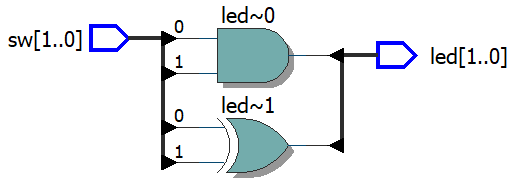
\includegraphics[scale=0.7]{elab1_1_rtl}
	\caption{Результат синтеза в RLT Viewer}
	\label{fig:elab1_1_rtl}
\end{center}
\end{figure}

\subsection{Результаты моделирования}
\label{sec:elab1_1_modeling}

На рис. \ref{fig:elab1_1_modeling} изображена временная диаграмма работы синтезированного устройства. На вход устройству поочередно подаются всевозможные комбинации значений \code{sw}.
\begin{figure}[H]
\begin{center}
	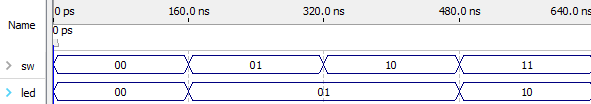
\includegraphics[width=\textwidth]{elab1_1_modeling}
	\caption{Результаты моделирования}
	\label{fig:elab1_1_modeling}
\end{center}
\end{figure}

\subsection{Назначение выводов СБИС}

На рис. \ref{fig:elab1_1_pins} приведены назначения выводов СБИС в Pin Planner.

\begin{figure}[H]
\begin{center}
	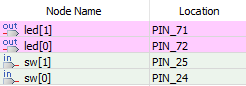
\includegraphics{elab1_1_pins}
	\caption{Таблица назначений в Pin Planer}
	\label{fig:elab1_1_pins}
\end{center}
\end{figure}

\subsection{Результаты проверки на плате}

Для тестирования проекта на плате были использованы тесты, описанные в пункте \ref{sec:elab1_1_modeling}. Результаты тестирования совпадают с ожидаемыми, следовательно, устройство работает верно.

\subsection{Выводы}

Разработан одноразрядный полусумматор. В описании использовались такие операторы, как Bitwise, Concatenate. Результаты моделирования и тестирования на плате показали, что разработанное устройство работает верно.

\newpage

\section{Полный одноразрядный сумматор}

\subsection{Задание}

На языке Verilog описать полный одноразрядный сумматор:
\begin{itemize}
	\item Входы:
	\begin{itemize}
		\item Данных - переключатели \code{sw[1:0]}.
		\item Переноса – кнопка \code{pba}.
	\end{itemize}
	\item Выходы – светодиоды \code{led[1:0]}.
\end{itemize}
В описании можно использовать операторы Bitwise, Logical, Reduction, Reduction, Replicator, Concatenate.

\subsection{Код на языке Verilog}

В листинге \ref{code:2} приведен код программы на языке Verilog.

\lstinputlisting[caption=elab1\_2.v, label=code:2]{elab1_2/elab1_2.v}

\subsection{Результаты синтеза}

На рис. \ref{fig:elab1_2_rtl} приведено изображение синтезированной схемы в RLT Viewer.

\begin{figure}[H]
\begin{center}
	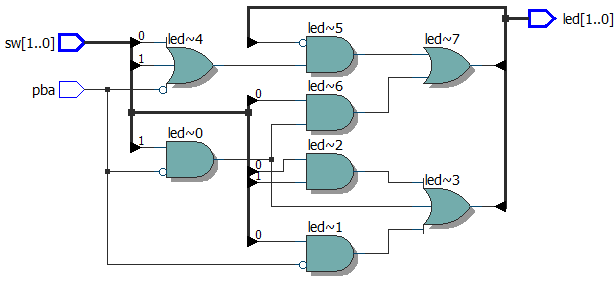
\includegraphics[scale=0.6]{elab1_2_rtl}
	\caption{Результат синтеза в RLT Viewer}
	\label{fig:elab1_2_rtl}
\end{center}
\end{figure}

\subsection{Результаты моделирования}
\label{sec:elab1_2_modeling}

На рис. \ref{fig:elab1_2_modeling} изображена временная диаграмма работы синтезированного устройства. На вход устройству поочередно подаются всевозможные комбинации значений \code{pba} (активный уровень 0) и \code{sw}.
\begin{figure}[H]
\begin{center}
	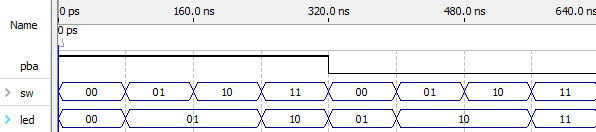
\includegraphics[width=\textwidth]{elab1_2_modeling}
	\caption{Результаты моделирования}
	\label{fig:elab1_2_modeling}
\end{center}
\end{figure}

\subsection{Назначение выводов СБИС}

На рис. \ref{fig:elab1_2_pins} приведены назначения выводов СБИС в Pin Planner.

\begin{figure}[H]
\begin{center}
	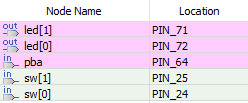
\includegraphics{elab1_2_pins}
	\caption{Таблица назначений в Pin Planer}
	\label{fig:elab1_2_pins}
\end{center}
\end{figure}

\subsection{Результаты проверки на плате}

Для тестирования проекта на плате были использованы тесты, описанные в пункте \ref{sec:elab1_2_modeling}. Результаты тестирования совпадают с ожидаемыми, следовательно, устройство работает верно.

\subsection{Выводы}

Разработан полный одноразрядный сумматор. В описании использовались такие операторы, как Bitwise, Concatenate. Результаты моделирования и тестирования на плате показали, что разработанное устройство работает верно.

\newpage

\section{Полный сумматор с последовательным переносом}

\subsection{Задание}

На языке Verilog опишите полный 2-х разрядный сумматор с последовательным переносом:
\begin{itemize}
	\item Входы:
	\begin{itemize}
		\item Данных - переключатели \code{sw[3:2]} и \code{sw[1:0]} соответственно.
		\item Переноса – кнопка \code{pba}.
	\end{itemize}
	\item Выходы – светодиоды \code{led[2:0]}.
\end{itemize}
В описании можно использовать операторы Bitwise, Logical, Reduction, Reduction, Replicator, Concatenate.

\subsection{Код на языке Verilog}

В листинге \ref{code:3} приведен код программы на языке Verilog.

\lstinputlisting[caption=elab1\_3.v, label=code:3]{elab1_3/elab1_3.v}

\subsection{Результаты синтеза}

На рис. \ref{fig:elab1_3_rtl} приведено изображение синтезированной схемы в RLT Viewer.

\begin{figure}[H]
\begin{center}
	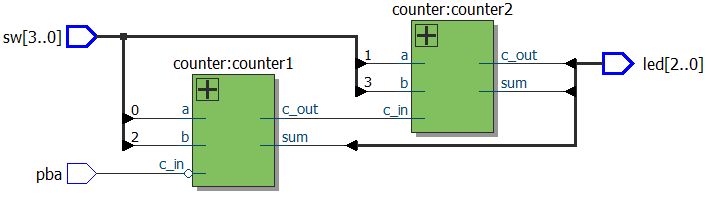
\includegraphics[scale=0.8]{elab1_3_rtl}
	\caption{Результат синтеза в RLT Viewer}
	\label{fig:elab1_3_rtl}
\end{center}
\end{figure}

\subsection{Результаты моделирования}
\label{sec:elab1_3_modeling}

На рис. \ref{fig:elab1_3_modeling} изображены временные диаграммы работы синтезированного устройства. На вход устройству поочередно подаются всевозможные комбинации значений \code{sw} при \code{pba = 1} (неактивный уровень) и при \code{pba = 0} (активный уровень) соответственно.
\begin{figure}[H]
\begin{center}
	\begin{subfigure}[b]{\textwidth}
		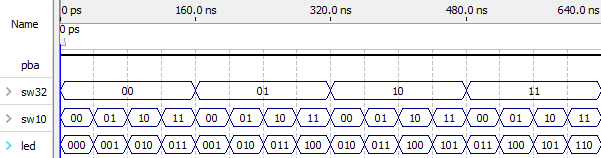
\includegraphics[width=\textwidth]{elab1_3_modeling_1}
	\end{subfigure}
	\begin{subfigure}[b]{\textwidth}
		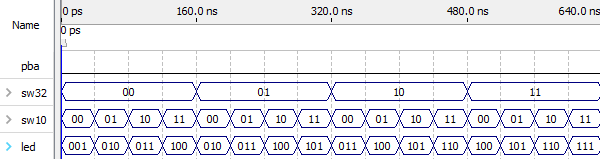
\includegraphics[width=\textwidth]{elab1_3_modeling_2}
	\end{subfigure}
	\caption{Результаты моделирования}
	\label{fig:elab1_3_modeling}
\end{center}
\end{figure}

\subsection{Назначение выводов СБИС}

На рис. \ref{fig:elab1_3_pins} приведены назначения выводов СБИС в Pin Planner.

\begin{figure}[H]
\begin{center}
	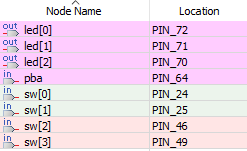
\includegraphics{elab1_3_pins}
	\caption{Таблица назначений в Pin Planer}
	\label{fig:elab1_3_pins}
\end{center}
\end{figure}

\subsection{Результаты проверки на плате}

Для тестирования проекта на плате были использованы тесты, описанные в пункте \ref{sec:elab1_3_modeling}. Результаты тестирования совпадают с ожидаемыми, следовательно, устройство работает верно.

\subsection{Выводы}

Разработан полный 2-х разрядный сумматор с последовательным переносом. В описании использовались такие операторы, как Bitwise, Concatenate. Результаты моделирования и тестирования на плате показали, что разработанное устройство работает верно.

\newpage

\lstset{inputpath={../lab2/quartus/}}
\graphicspath{{../lab2/pics/}}

\section{Беззнаковый делитель с повышенной точностью}

\subsection{Задание}

На языке Verilog опишите беззнаковый делитель с повышенной точностью (4 знака после запятой):
\begin{itemize}
\item Входы
	\begin{itemize}
		\item Делимое - переключатели \code{sw[7:4]};
		\item Делитель - переключатели \code{sw[3:0]}.
	\end{itemize}
\item Выходы
	\begin{itemize}
		\item Результат деления - светодиоды \code{led[7:4]};
		\item Знаки после запятой – светодиоды \code{led[3:0]}.
	\end{itemize}
\end{itemize}

В описании можно использовать любые операторы. Тип данных - \code{wire}.

\subsection{Код на языке Verilog}

В листинге \ref{code:4} приведен код программы на языке Verilog.

\lstinputlisting[caption=elab2\_1.v, label=code:4]{elab2_1/elab2_1.v}

\subsection{Результаты синтеза}

На рис. \ref{fig:elab2_1_rtl} приведено изображение синтезированной схемы в RLT Viewer.

\begin{figure}[H]
\begin{center}
	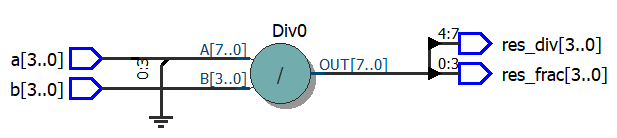
\includegraphics[scale=0.8]{elab2_1_rtl}
	\caption{Результат синтеза в RLT Viewer}
	\label{fig:elab2_1_rtl}
\end{center}
\end{figure}

\subsection{Результаты моделирования}
\label{sec:elab2_1_modeling}

На рис. \ref{fig:elab2_1_modeling} изображена временная диаграмма работы синтезированного устройства. На вход устройству поочередно подаются случайные без знаковые значения \code{a[3:0]} и \code{b[3:0]}, результат деления записывается в \code{res_div[3:0]}, а знаки после запятой в \code{res_frac[3:0]}.
\begin{figure}[H]
\begin{center}
	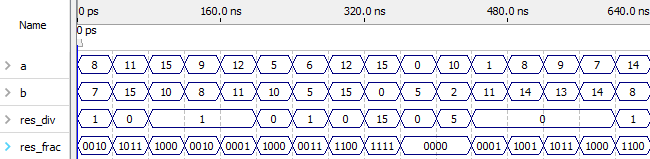
\includegraphics[width=\textwidth]{elab2_1_modeling}
	\caption{Результаты моделирования}
	\label{fig:elab2_1_modeling}
\end{center}
\end{figure}

\subsection{Назначение выводов СБИС}

На рис. \ref{fig:elab2_1_pins} приведены назначения выводов СБИС в Pin Planner.

\begin{figure}[H]
\begin{center}
	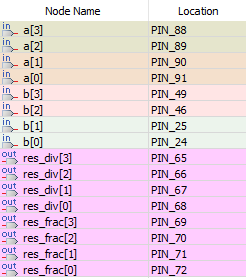
\includegraphics{elab2_1_pins}
	\caption{Таблица назначений в Pin Planer}
	\label{fig:elab2_1_pins}
\end{center}
\end{figure}

\subsection{Результаты проверки на плате}

Для тестирования проекта на плате были использованы тесты, описанные в пункте \ref{sec:elab2_1_modeling}. Результаты тестирования совпадают с ожидаемыми, следовательно, устройство работает верно.

\subsection{Выводы}

Разработан без знаковый делитель с повышенной точностью. Результаты моделирования и тестирования на плате показали, что разработанное устройство работает верно.

\newpage

\section{Знаковый умножитель на фиксированное число}

\subsection{Задание}

\noindent На языке Verilog опишите знаковый умножитель на фиксированное число:
\begin{itemize}
	\item Множитель равен 9.
	\item Входы данных - переключатели \code{sw[3:0]} соответственно.
	\item Выходы – светодиоды \code{led[7:0]}.
\end{itemize}

\noindent В описании можно использовать операторы сдвига, сложения, вычитания, Replicator, Concatenate.

\subsection{Код на языке Verilog}

В листинге \ref{code:5} приведен код программы на языке Verilog.

\lstinputlisting[caption=elab2\_2.v, label=code:5]{elab2_2/elab2_2.v}

\subsection{Результаты синтеза}

На рис. \ref{fig:elab2_2_rtl} приведено изображение синтезированной схемы в RLT Viewer.

\begin{figure}[H]
\begin{center}
	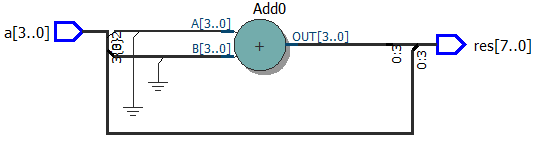
\includegraphics[scale=0.9]{elab2_2_rtl}
	\caption{Результат синтеза в RLT Viewer}
	\label{fig:elab2_2_rtl}
\end{center}
\end{figure}

\subsection{Результаты моделирования}
\label{sec:elab2_2_modeling}

На рис. \ref{fig:elab2_2_modeling} изображена временная диаграмма работы синтезированного устройства. На вход устройству поочередно подаются случайное знаковое значение \code{a[3:0]}, а результат умножения записывается в \code{res[7:0]}.

\begin{figure}[H]
\begin{center}
	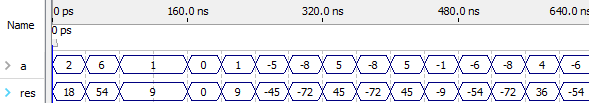
\includegraphics[width=\textwidth]{elab2_2_modeling}
	\caption{Результаты моделирования}
	\label{fig:elab2_2_modeling}
\end{center}
\end{figure}

\subsection{Назначение выводов СБИС}

На рис. \ref{fig:elab2_2_pins} приведены назначения выводов СБИС в Pin Planner.

\begin{figure}[H]
\begin{center}
	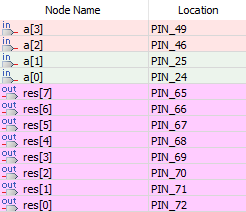
\includegraphics{elab2_2_pins}
	\caption{Таблица назначений в Pin Planer}
	\label{fig:elab2_2_pins}
\end{center}
\end{figure}

\subsection{Результаты проверки на плате}

Для тестирования проекта на плате были использованы тесты, описанные в пункте \ref{sec:elab2_2_modeling}. Результаты тестирования совпадают с ожидаемыми, следовательно, устройство работает верно.

\subsection{Выводы}

Разработан знаковый умножитель на фиксированное число. Результаты моделирования и тестирования на плате показали, что разработанное устройство работает верно.

\newpage

\lstset{inputpath={../lab3/quartus/}}
\graphicspath{{../lab3/pics/}}

\section{Преобразователь двоичного кода в код Грея}

\subsection{Задание}

На языке Verilog опишите преобразователь 4-х разрядного двоичного кода в код Грея:
\begin{itemize}
	\item Входы: переключатели \code{sw[3:0]} -- 4-х разрядный двоичный код.
	\item Выходы: светодиоды \code{led[3:0]} –- код Грея.
\end{itemize}

В описании можно использовать операторы Bitwise, Logical, Reduction, Reduction, Replicator, Concatenate. Тип данных -- \code{wire}.

\subsection{Код на языке Verilog}

В листинге \ref{code:6} приведен код программы на языке Verilog.

\lstinputlisting[caption=elab3\_1.v, label=code:6]{elab3_1/elab3_1.v}

\subsection{Результаты синтеза}

На рис. \ref{fig:elab3_1_rtl} приведено изображение синтезированной схемы в RLT Viewer.

\begin{figure}[H]
\begin{center}
	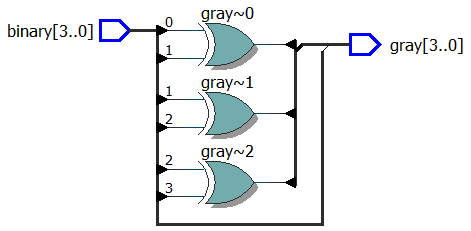
\includegraphics[scale=0.9]{elab3_1_rtl}
	\caption{Результат синтеза в RLT Viewer}
	\label{fig:elab3_1_rtl}
\end{center}
\end{figure}

\subsection{Результаты моделирования}
\label{sec:elab3_1_modeling}

На рис. \ref{fig:elab3_1_modeling} изображена временная диаграмма работы синтезированного устройства. На вход устройства поочередно подаются всевозможные значения \code{binary[3:0]}, соответствующие числам от \code{0} до \code{15}, а преобразованное значение в код Грея записывается в \code{gray[3:0]}.

\begin{figure}[H]
\begin{center}
	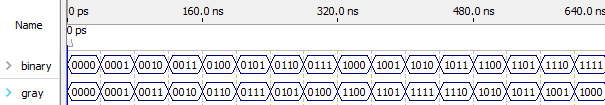
\includegraphics[width=\textwidth]{elab3_1_modeling}
	\caption{Результаты моделирования}
	\label{fig:elab3_1_modeling}
\end{center}
\end{figure}

\subsection{Назначение выводов СБИС}

На рис. \ref{fig:elab3_1_pins} приведены назначения выводов СБИС в Pin Planner.

\begin{figure}[H]
\begin{center}
	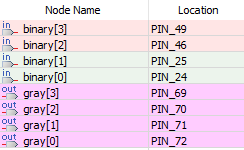
\includegraphics{elab3_1_pins}
	\caption{Таблица назначений в Pin Planer}
	\label{fig:elab3_1_pins}
\end{center}
\end{figure}

\subsection{Результаты проверки на плате}

Для тестирования проекта на плате были использованы тесты, описанные в пункте \ref{sec:elab3_1_modeling}. Результаты тестирования совпадают с ожидаемыми, следовательно, устройство работает верно.

\subsection{Выводы}

Реализован преобразователь 4-х разрядного двоичного кода в код Грея. Результаты моделирования и тестирования на плате показали, что разработанное устройство работает верно.

\section{Преобразователь кода Грея в двоичный код}

\subsection{Задание}

На языке Verilog опишите преобразователь 4-х разрядного кода Грея в двоичный код:
\begin{itemize}
	\item Входы: переключатели \code{sw[3:0]} -- 4-х разрядный код Грея.
	\item Выходы: светодиоды \code{led[3:0]} -– двоичный код.
\end{itemize}

В описании можно использовать операторы Bitwise, Logical, Reduction, Reduction, Replicator, Concatenate. Тип данных - \code{wire}.

\subsection{Код на языке Verilog}

В листинге \ref{code:7} приведен код программы на языке Verilog.

\lstinputlisting[caption=elab3\_2.v, label=code:7]{elab3_2/elab3_2.v}

\subsection{Результаты синтеза}

На рис. \ref{fig:elab3_2_rtl} приведено изображение синтезированной схемы в RLT Viewer.

\begin{figure}[H]
\begin{center}
	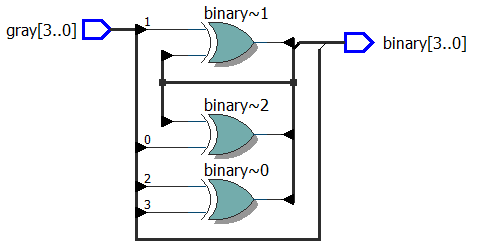
\includegraphics[scale=0.9]{elab3_2_rtl}
	\caption{Результат синтеза в RLT Viewer}
	\label{fig:elab3_2_rtl}
\end{center}
\end{figure}

\subsection{Результаты моделирования}
\label{sec:elab3_2_modeling}

На рис. \ref{fig:elab3_2_modeling} изображена временная диаграмма работы синтезированного устройства. На вход устройства поочередно подаются всевозможные значения \code{gray[3:0]}, соответствующие числам от \code{0} до \code{15}, а преобразованное значение в код Грея записывается в \code{binary[3:0]}.

\begin{figure}[H]
\begin{center}
	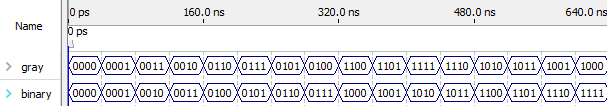
\includegraphics[width=\textwidth]{elab3_2_modeling}
	\caption{Результаты моделирования}
	\label{fig:elab3_2_modeling}
\end{center}
\end{figure}

\subsection{Назначение выводов СБИС}

На рис. \ref{fig:elab3_2_pins} приведены назначения выводов СБИС в Pin Planner.

\begin{figure}[H]
\begin{center}
	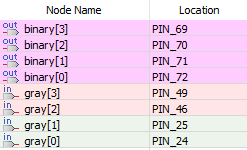
\includegraphics{elab3_2_pins}
	\caption{Таблица назначений в Pin Planer}
	\label{fig:elab3_2_pins}
\end{center}
\end{figure}

\subsection{Результаты проверки на плате}

Для тестирования проекта на плате были использованы тесты, описанные в пункте \ref{sec:elab3_2_modeling}. Результаты тестирования совпадают с ожидаемыми, следовательно, устройство работает верно.

\subsection{Выводы}

Реализован преобразователь 4-х разрядного кода Грея в двоичный код. Результаты моделирования и тестирования на плате показали, что разработанное устройство работает верно.

\newpage

\lstset{inputpath={../lab4/quartus/}}
\graphicspath{{../lab4/pics/}}

\section{Реверсивный счетчик с динамически изменяемым модулем счета}

\subsection{Задание}

На языке Verilog опишите устройство, включающее:
\begin{itemize}
	\item Счетчик-делитель, обеспечивающий счет по модулю \code{25 000 000} и формирующий синхронный сигнал переноса (активный уровень сигнала \code{= 1}, длительность один такт тактовой частоты) по достижению счетчиком значения \code{25 000 000 - 1}.
	\item 8-разрядный реверсивный счетчик с динамически изменяемым модулем счета. Вход модуля счета счетчика \code{mod[7:0]} -- соединен с входами \code{sw[7:0]} устройства. Сигналы управления счетчиком заданы приведенной ниже таблицей.
\vspace{-0.5cm}
\begin{table}[H]
\begin{center}
	\def\tabcolsep{13pt}
	\caption{Алгоритм работы счетчика}
	\begin{tabular}{|c|c|c|c|c|}
	\hline	
	\code{ena} & \code{load} & \code{dir} & \code{q} \\ 
	\hline
	\code{0} & \code{X} & \code{X} & Хранение \\
	\hline
	\code{1} & \code{1} & \code{X} & Синхронная загрузка \\
	\hline
	\code{1} & \code{0} & \code{1} & Счет \code{+} \\
	\hline
	\code{1} & \code{0} & \code{0} & Счет \code{-} \\
	\hline
	\end{tabular}
\end{center}
\end{table}	
\vspace{-0.5cm}
	\item Модуль формирования сигнала \code{load} для 8-разрядного реверсивного счетчика -- сигнал \code{load = 1} длительностью \code{1} период тактового сигнала \code{clk} формируется при изменении значения модуля счета, заданного на входах \code{sw[7:0]} устройства.

	\item Входы:
		\begin{itemize}
			\item Переключатели \code{sw[7:0]} -- модуль счета счетчика.
			\item Кнопка \code{pbb} -- кнопка выбора направления счета (если \code{pbb} нажата, то счет на вычитание).
			\item Тактовый сигнал (\code{clk}) подается от тактового генератора (см. описание стенда). Частота тактового сигнала – 25МГц.
		\end{itemize}
	\item Выходы: светодиоды \code{led[7:0]} (выходы двоичного 8-разрядного счетчика).
\end{itemize}

Дополнительные требования:
\begin{itemize}
	\item[$\circ$] Счетчик-делитель, 8-разрядный реверсивный счетчик и модуль формирования сигнала \code{load} описываются в отдельных процедурных блоках.
	\item[$\circ$] При моделировании устройства, с целью сокращения времени моделирования, для счетчика-делителя установите коэффициент деления частоты равным \code{3} (а не \code{25 000 000}).
	\item[$\circ$] На результатах моделирования должны отображаться, кроме всех входных сигналов: значение счетчика-делителя, сигнал переноса, значение 8-разрядного реверсивного счетчика, сигнал \code{load}.
\end{itemize}

В описании можно использовать любые операторы.

\subsection{Код на языке Verilog}

В листинге \ref{code:8} приведен код программы на языке Verilog.

\lstinputlisting[caption=elab4\_1.v, label=code:8]{elab4_1/elab4_1.v}

\subsection{Результаты синтеза}

На рис. \ref{fig:elab4_1_rtl} приведено изображение синтезированной схемы в RLT Viewer.

\begin{figure}[H]
\begin{center}
	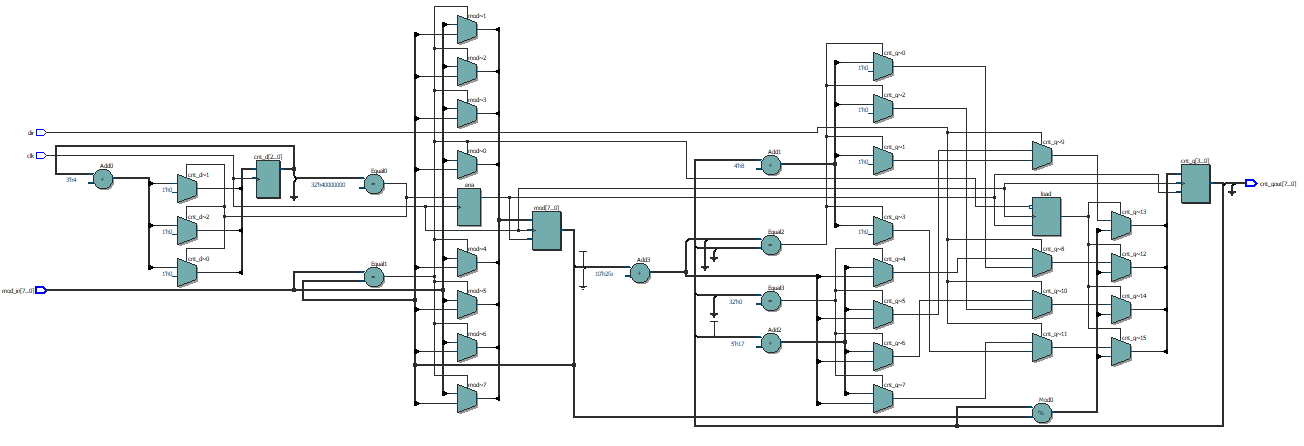
\includegraphics[width=\textwidth]{elab4_1_rtl}
	\caption{Результат синтеза в RLT Viewer}
	\label{fig:elab4_1_rtl}
\end{center}
\end{figure}

\subsection{Результаты моделирования}
\label{sec:elab4_1_modeling}

На рис. \ref{fig:elab4_1_modeling} изображена временная диаграмма работы синтезированного устройства. 

\begin{figure}[H]
\begin{center}
	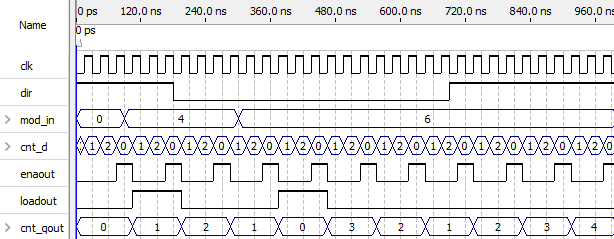
\includegraphics[width=\textwidth]{elab4_1_modeling}
	\caption{Результаты моделирования}
	\label{fig:elab4_1_modeling}
\end{center}
\end{figure}

\subsection{Назначение выводов СБИС}

На рис. \ref{fig:elab4_1_pins} приведены назначения выводов СБИС в Pin Planner.

\begin{figure}[H]
\begin{center}
	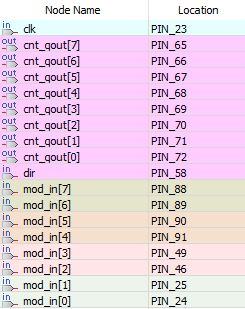
\includegraphics{elab4_1_pins}
	\caption{Таблица назначений в Pin Planer}
	\label{fig:elab4_1_pins}
\end{center}
\end{figure}

\subsection{Результаты проверки на плате}

Для тестирования проекта на плате были использованы тесты, описанные в пункте \ref{sec:elab4_1_modeling}. Результаты тестирования совпадают с ожидаемыми, следовательно, устройство работает верно.

\subsection{Выводы}

Реализовано устройство, содержащее счетчик-делитель и 8-разрядный реверсивный счетчик с динамически изменяемым модулем счета. Результаты моделирования и тестирования на плате показали, что разработанное устройство работает верно.

\newpage

\lstset{inputpath={../lab5/quartus/}}
\graphicspath{{../lab5/pics/}}

\section{Параметризированное АЛУ}

\subsection{Задание}

На языке Verilog опишите устройство, включающее:
\begin{itemize}
	\item Два входа операндов (\code{op_a}, \code{op_b}) -- операнды без знаковые.
	\item Вход кода операции (\code{op}).
	\item Выход результата (\code{res}).
	\item Выход переполнения (\code{over}).
	\item Параметр: \code{N} -- разрядность операндов и результата (базовое значение 3).
	\item Локальный параметр: \code{code_op} -- код операции.
	\vspace{-0.5cm}
	\begin{table}[H]
	\begin{center}
		\def\tabcolsep{10pt}
		\caption{Коды операций}
		\begin{tabular}{|c|c|c|c|c|}
		\hline	
		\makecell{Обозначение \\ кода операции} & \makecell{Значение \\ кода операции} & Операция \\ 
		\hline
		\code{ZERO} & \code{00} & \code{res = 0} \\
		\hline
		\code{SUM} & \code{01} & \code{res = op_a + op_b} \\
		\hline
		\code{SUB} & \code{10} & \code{res = op_a - op_b} \\
		\hline
		\code{MULT} & \code{11} & На выходе большее из \code{op_a} и \code{op_b} \\
		\hline
		\end{tabular}
	\end{center}
	\end{table}	
	\vspace{-0.5cm}
	\item Входы:
		\begin{itemize}
			\item Переключатели \code{sw[2:0]} -- операнд А (\code{op_a})
			\item Переключатели \code{sw[5:3]} -- операнд В (\code{op_b})
			\item Переключатели \code{sw[7:6]} -- код операции (\code{op})
		\end{itemize}
	\item Выходы:
		\begin{itemize}
			\item Светодиоды \code{led[2:0]} -- выход результата (\code{res});
			\item светодиод \code{led[3]} -- выход переполнения (\code{over}).
		\end{itemize}
\end{itemize}

Дополнительные требования:
\begin{itemize}
	\item[$\circ$] Стандарты и номера выводов СБИС для платы miniDiLaB\_CIV задать с помощью атрибутов.
	\item[$\circ$] Осуществите функциональное моделирование (и приведите в отчете результаты) при \code{N = 8}.
	\item[$\circ$] Проверку на плате осуществите при \code{N = 3}.
\end{itemize}

В описании можно использовать любые операторы.

\subsection{Код на языке Verilog}

В листинге \ref{code:9} приведен код программы на языке Verilog.

\lstinputlisting[caption=elab5\_1.v, label=code:9]{elab5_1/elab5_1.v}

\newpage

\subsection{Результаты синтеза}

На рис. \ref{fig:elab5_1_rtl} приведено изображение синтезированной схемы в RLT Viewer.

\begin{figure}[H]
\begin{center}
	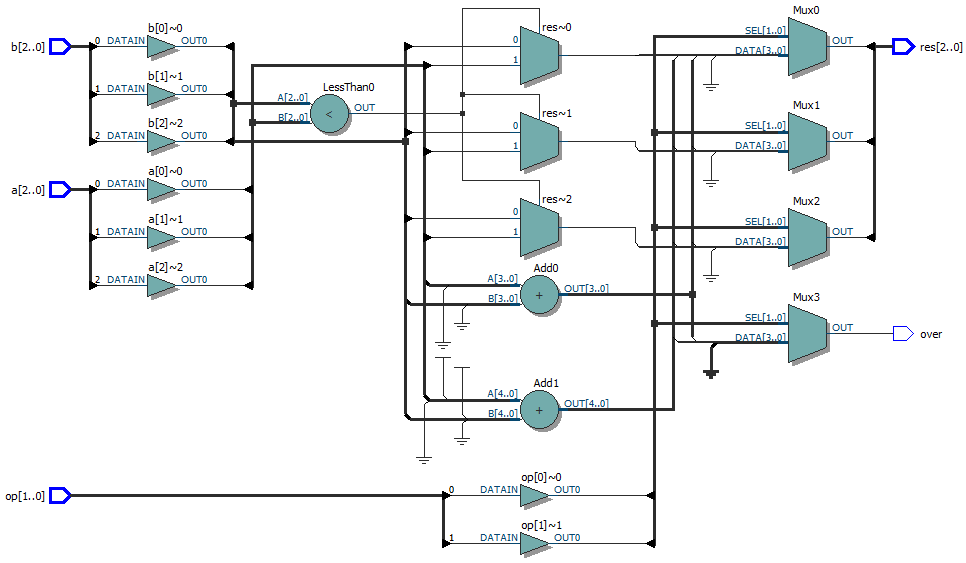
\includegraphics[width=\textwidth]{elab5_1_rtl}
	\caption{Результат синтеза в RLT Viewer}
	\label{fig:elab5_1_rtl}
\end{center}
\end{figure}

\subsection{Результаты моделирования}
\label{sec:elab5_1_modeling}

На рис. \ref{fig:elab5_1_modeling} изображена временная диаграмма работы синтезированного устройства. 

\begin{figure}[H]
\begin{center}
	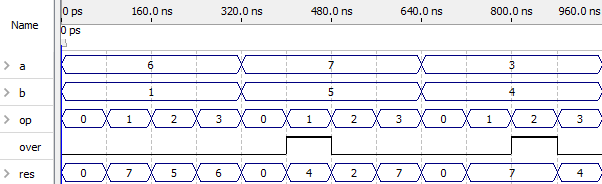
\includegraphics[width=\textwidth]{elab5_1_modeling}
	\caption{Результаты моделирования}
	\label{fig:elab5_1_modeling}
\end{center}
\end{figure}

\subsection{Назначение выводов СБИС}

На рис. \ref{fig:elab5_1_pins} приведены назначения выводов СБИС в Pin Planner.

\begin{figure}[H]
\begin{center}
	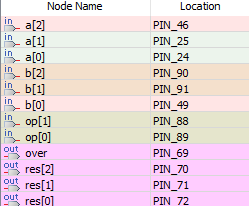
\includegraphics{elab5_1_pins}
	\caption{Таблица назначений в Pin Planer}
	\label{fig:elab5_1_pins}
\end{center}
\end{figure}

\subsection{Результаты проверки на плате}

Для тестирования проекта на плате были использованы тесты, описанные в пункте \ref{sec:elab5_1_modeling}. Результаты тестирования совпадают с ожидаемыми, следовательно, устройство работает верно.

\subsection{Выводы}

Реализовано устройство, принимающее на вход два операнда и код операции и вычисляющее результат. Результаты моделирования и тестирования на плате показали, что разработанное устройство работает верно.

\newpage

\section{Конечный автомат на основе счетчика}

\subsection{Задание}

На языке Verilog опишите устройство, включающее:
\begin{itemize}
	\item Счетчик-делитель, обеспечивает счет по модулю \code{N} (базовое значение -- 3) и формирование синхронного сигнала переноса (активный уровень сигнала -- 1, длительность один такт тактовой частоты) по достижению счетчиком значения \code{N-1}.
	\item Модуль, алгоритм которого задан графом переходов на рис. \ref{fig:lab5_2_0}.
		\vspace{-0.5cm}
		\begin{figure}[H]
		\begin{center}
			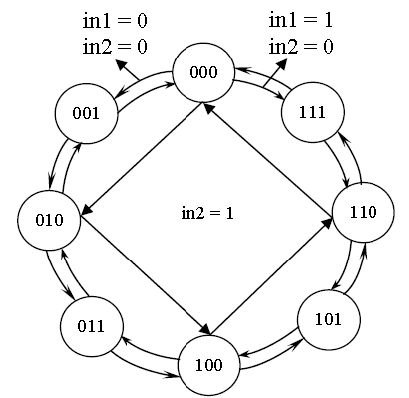
\includegraphics[scale=0.7]{lab5_2_0}
			\caption{Конечный автомат}
			\label{fig:lab5_2_0}
		\end{center}
		\end{figure}
		\vspace{-1cm}
		\begin{itemize}
			\item \code{in1}, \code{in2} -- входные сигналы модуля;
			\item Модуль имеет вход асинхронного сброса (сигнал \code{rst}) в состояние, в котором выходные сигналы \code{000}: при \code{rst=0} -- асинхронный сброс;
			\item Модуль имеет вход разрешения работы -- \code{ena} (при \code{ena=1} -- работа разрешена), подключенный к сигналу переноса счетчика-делителя.
		\end{itemize}
	\item Входы:
		\begin{itemize}
			\item Переключатель \code{sw[1]} -- вход \code{in1};
			\item Переключатель \code{sw[2]} – вход \code{in2};
			\item Кнопка \code{pba} – вход асинхронного сброса (кнопка нажата – сброс);
			\item Тактовый сигнал (\code{clk}) подается от тактового генератора (см. описание стенда). Частота тактового сигнала – 25МГц.
		\end{itemize}
	\item Выходы: светодиоды \code{led[2:0]} -- выходы модуля.
\end{itemize}
В описании можно использовать любые операторы.

\subsection{Код на языке Verilog}

В листинге \ref{code:10} приведен код программы на языке Verilog.

\lstinputlisting[caption=elab5\_1.v, label=code:10]{elab5_2/elab5_2.v}

\subsection{Результаты синтеза}

На рис. \ref{fig:elab5_2_rtl} приведено изображение синтезированной схемы в RLT Viewer.

\begin{figure}[H]
\begin{center}
	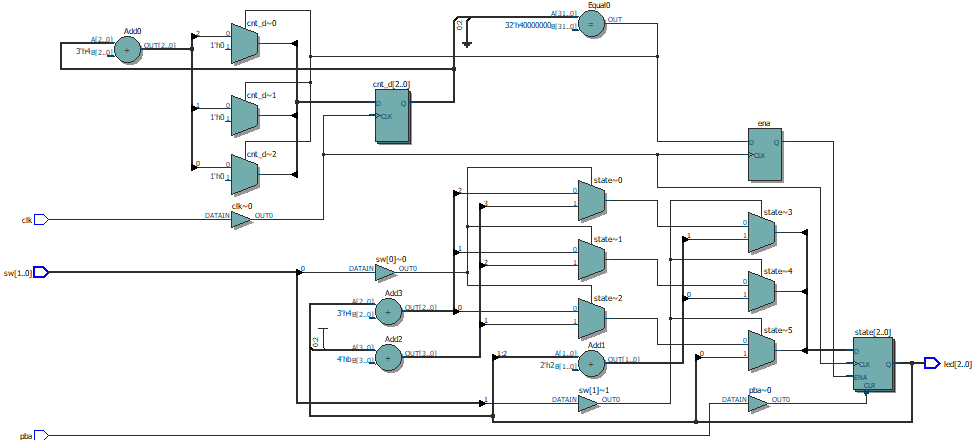
\includegraphics[width=\textwidth]{elab5_2_rtl}
	\caption{Результат синтеза в RLT Viewer}
	\label{fig:elab5_2_rtl}
\end{center}
\end{figure}

\subsection{Результаты моделирования}
\label{sec:elab5_2_modeling}

На рис. \ref{fig:elab5_2_modeling} изображена временная диаграмма работы синтезированного устройства. 

\begin{figure}[H]
\begin{center}
	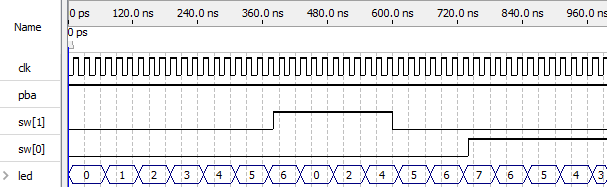
\includegraphics[width=\textwidth]{elab5_2_modeling}
	\caption{Результаты моделирования}
	\label{fig:elab5_2_modeling}
\end{center}
\end{figure}

\newpage

\subsection{Назначение выводов СБИС}

На рис. \ref{fig:elab5_2_pins} приведены назначения выводов СБИС в Pin Planner.

\begin{figure}[H]
\begin{center}
	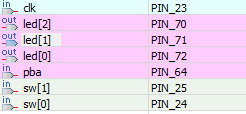
\includegraphics{elab5_2_pins}
	\caption{Таблица назначений в Pin Planer}
	\label{fig:elab5_2_pins}
\end{center}
\end{figure}

\subsection{Результаты проверки на плате}

Для тестирования проекта на плате были использованы тесты, описанные в пункте \ref{sec:elab5_2_modeling}. Результаты тестирования совпадают с ожидаемыми, следовательно, устройство работает верно.

\subsection{Выводы}

Реализовано устройство, принимающее на вход два операнда и код операции и вычисляющее результат. Результаты моделирования и тестирования на плате показали, что разработанное устройство работает верно.

\newpage

\lstset{inputpath={../lab6/quartus/}}
\graphicspath{{../lab6/pics/}}

\section{N-разрядный последовательный умножитель}

\subsection{Задание}

На языке Verilog создайте параметризированное описание N-разрядного последовательного умножителя, осуществляющего умножение по алгоритму:
\begin{itemize}
	\item Умножение старшими разрядами вперед со сдвигом суммы.
	\item Параметр \code{N} -- разрядность входных данных (по умолчанию задайте его равным 8) -- операндов.
	\item Параметр \code{INV} -- инверсия выходных данных умножителя ($=1$ выходные данные инвертируются; $=0$ выходные данные не инвертируются).
	\item Загрузка в умножитель новых значений операндов и запуск процедуры умножения должны происходить при изменении любого из операндов:
		\begin{itemize}
			\item При изменении любого из операндов должен формироваться логический аналог сигнала \code{load}, приведенного в примере;
			\item Подсказка: для каждого операнда потребуется регистр для хранения предыдущего значения операнда, которое будет сравниваться с текущим значением операнда.
		\end{itemize}
	\item Входы:
		\begin{itemize}
			\item Переключатель \code{sw[7:4]} -- операнд В -- множимое;
			\item Переключатель \code{sw[3:0]} -- операнд А -- множитель.
		\end{itemize}
	\item Выходы: светодиоды \code{led[7:0]} – выходы умножителя.
\end{itemize}

Дополнительные требования:
\begin{itemize}
	\item[$\circ$] Стандарты и номера выводов СБИС для платы miniDiLaB\_CIV задать с помощью атрибутов.
	\item[$\circ$] Осуществите функциональное моделирование (и приведите в отчете результаты) при: \code{N = 8; INV = 0}.
	\item[$\circ$] Проверку на плате осуществите при: \code{N = 4; INV = 1}.
\end{itemize}
В описании можно использовать любые операторы.

\newpage

\subsection{Код на языке Verilog}

В листинге \ref{code:11} приведен код программы на языке Verilog.

\lstinputlisting[caption=elab6\_1.v, label=code:11]{elab6_1/elab6_1.v}

\subsection{Результаты синтеза}

На рис. \ref{fig:elab6_1_rtl} приведено изображение синтезированной схемы в RLT Viewer при \code{N = 2; INV = 0}.

\begin{figure}[H]
\begin{center}
	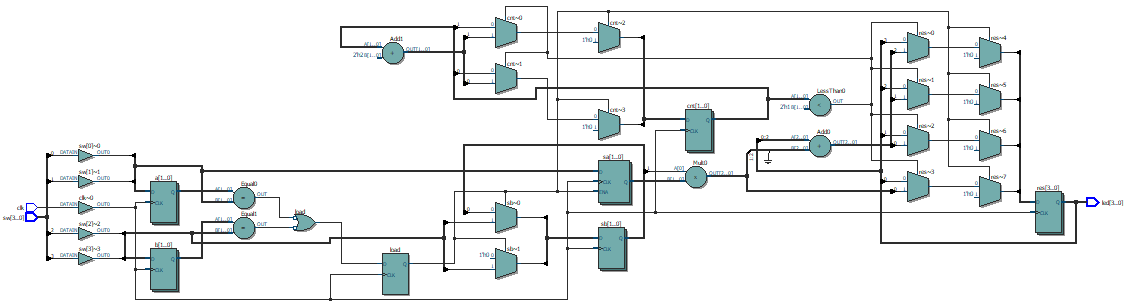
\includegraphics[width=\textwidth]{elab6_1_rtl}
	\caption{Результат синтеза в RLT Viewer}
	\label{fig:elab6_1_rtl}
\end{center}
\end{figure}

\subsection{Результаты моделирования}
\label{sec:elab6_1_modeling}

На рис. \ref{fig:elab6_1_modeling} изображена временная диаграмма работы синтезированного устройства при \code{N = 8; INV = 0}. На вход подаются случайные значения множимого \code{inb[7:0]} и множителя \code{ina[7:0]}, а результат записывается в \code{led[15:0]}.

\begin{figure}[H]
\begin{center}
	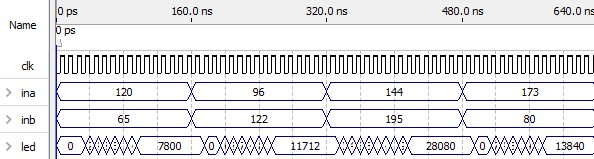
\includegraphics[width=\textwidth]{elab6_1_modeling}
	\caption{Результаты моделирования}
	\label{fig:elab6_1_modeling}
\end{center}
\end{figure}

\newpage

\subsection{Назначение выводов СБИС}

На рис. \ref{fig:elab6_1_pins} приведены назначения выводов СБИС в Pin Planner.

\begin{figure}[H]
\begin{center}
	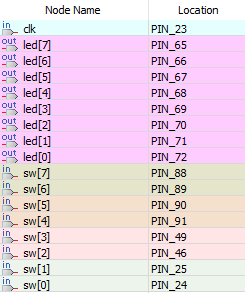
\includegraphics{elab6_1_pins}
	\caption{Таблица назначений в Pin Planer}
	\label{fig:elab6_1_pins}
\end{center}
\end{figure}

\subsection{Результаты проверки на плате}

Для тестирования проекта на плате были использованы тесты, описанные в пункте \ref{sec:elab6_1_modeling} при параметрах \code{N = 4; INV = 1}. Результаты тестирования совпадают с ожидаемыми, следовательно, устройство работает верно.

\subsection{Выводы}

Реализовано параметризированное описание N-разрядного последовательно умножителя, осуществляющего умножение по алгоритму старшими разрядами вперед со сдвигом суммы. Результаты моделирования и тестирования на плате показали, что разработанное устройство работает верно.

\newpage

\lstset{inputpath={../lab7/quartus/}}
\graphicspath{{../lab7/pics/}}

\section{Параметризированное устройство с модулем памяти}

\subsection{Задание}

На языке Verilog создайте структурное описание параметризированного устройства (параметр \code{INV = 1} -- инверсия выходных данных), приведенного на рис. \ref{fig:elab7_1_0}.

\begin{figure}[H]
\begin{center}
	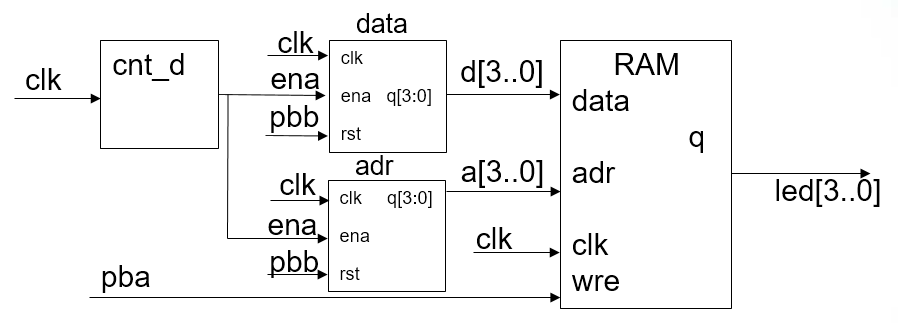
\includegraphics[width=\textwidth]{elab7_1_0}
	\caption{Параметризированное устройство}
	\label{fig:elab7_1_0}
\end{center}
\end{figure}
\vspace{-0.5cm}

В состав устройства входят:
\begin{itemize}
	\item \code{cnt_d} -- cчетчик делитель (параметр -- \code{DIV}), обеспечивающий счет по модулю \code{DIV} (базовое значение -- $3$) и формирование синхронного сигнала переноса (активный уровень сигнала -- $1$, длительность один такт тактовой частоты) по достижению счетчиком значения \code{DIV - 1}.
	\item \code{data} -- формирователь данных для модуля памяти (реализован на базе параметризированного счетчика \code{cnt_N}).
	\item \code{adr} -- формирователь адреса для модуля памяти (реализован на базе параметризированного счетчика \code{cnt_N}).
	\item \code{RAM} -- модуль памяти (параметры: \code{word_num} -- число слов (базовое значение $16$), \code{data_W} -- разрядность данных (базовое значение $4$); простая одно портовая память с чтением новых данных в процессе записи):
		\begin{itemize}
			\item Для расчета разрядности шины адреса следует использовать функцию с постоянным значением для вычисления $\log_2($\code{word_num}$)$;
			\item Вход \code{wre} – вход разрешения записи ($=1$ -- запись в память разрешена);
			\item Модуль памяти должен быть инициализирован данными: \code{4'h0} -- четные адреса; \code{4'hf} -- нечетные адреса.
		\end{itemize}
	\item \code{cnt_N} -- двоичный счетчик на сложение с параметризированной разрядностью (параметр \code{N}, базовое значение -- $4$), имеющий вход тактовых сигналов (\code{clk}), вход разрешения работы (\code{ena}), вход асинхронного сброса (\code{rst}) и выход -- \code{q[N-1:0]}.
	\item Входы:
		\begin{itemize}
			\item Кнопка \code{pbb} -- вход асинхронного сброса (кнопка нажата – сброс);
			\item Кнопка \code{pba} -- вход разрешения записи в память (кнопка нажата – запись разрешена);
			\item Тактовый сигнал (\code{clk}) подается от тактового генератора. Частота тактового сигнала -- 25МГц.
		\end{itemize}
	\item Выходы: светодиоды \code{led[3:0]} -- выходы устройства.
\end{itemize}

Дополнительные требования:
\begin{itemize}
	\item[$\circ$] Стандарты и номера выводов СБИС для платы miniDiLaB\_CIV задать с помощью атрибутов.
	\item[$\circ$] Осуществите функциональное моделированиеми  модулей \code{cnt_d}, \code{cnt_N}, \code{RAM} с базовыми значениями параметров.
	\item[$\circ$] Осуществите функциональное моделирование устройства при: \code{DIV = 3}, \code{N = 4}, \code{word_num = 16}, \code{data_W = 4}, \code{INV = 0}.
	\item[$\circ$] Проверку устройства на плате осуществите при: \code{DIV = 25_000_000}, \code{N = 4}, \code{word_num = 16}, \code{data_W = 4}, \code{INV = 1}.
\end{itemize}
В описании можно использовать любые операторы.

\newpage

\subsection{Код на языке Verilog}

В листингах \ref{code:12} -- \ref{code:15} приведен код программы на языке Verilog.

\lstinputlisting[caption=elab7\_1.v, label=code:12]{elab7_1/elab7_1.v}

\newpage

\lstinputlisting[caption=cnt\_d.v, label=code:13]{elab7_1/cnt_d.v}

\lstinputlisting[caption=cnt\_N.v, label=code:14]{elab7_1/cnt_N.v}

\newpage

\lstinputlisting[caption=RAM.v, label=code:15]{elab7_1/RAM.v}

\newpage

\subsection{Результаты синтеза}

На рис. \ref{fig:elab7_1_rtl} -- \ref{fig:elab7_1_rtl_3} приведены изображения синтезированного устройства и каждого модуля по отдельности в RLT Viewer.

\begin{figure}[H]
\begin{center}
	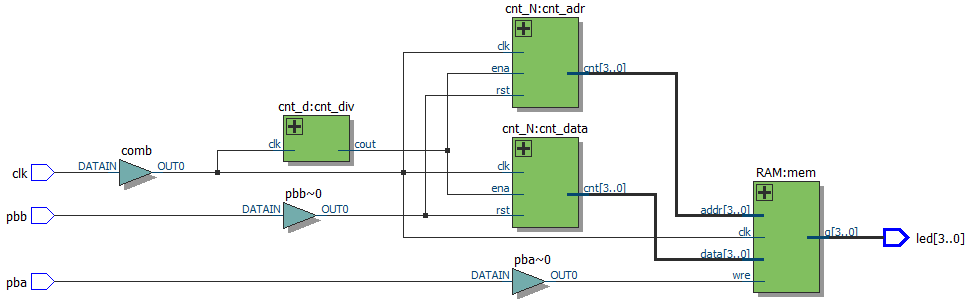
\includegraphics[width=\textwidth]{elab7_1_rtl}
	\caption{Результат синтеза устройства в RLT Viewer}
	\label{fig:elab7_1_rtl}
\end{center}
\end{figure}

\begin{figure}[H]
\begin{center}
	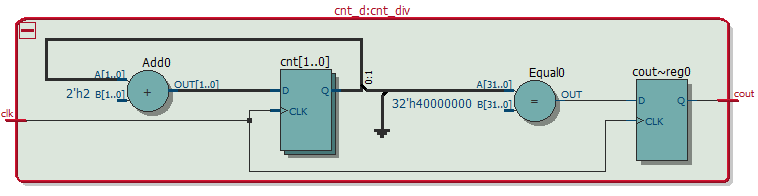
\includegraphics[width=\textwidth]{elab7_1_rtl_1}
	\caption{Результат синтеза \code{cnt_div} в RLT Viewer}
	\label{fig:elab7_1_rtl_1}
\end{center}
\end{figure}

\begin{figure}[H]
\begin{center}
	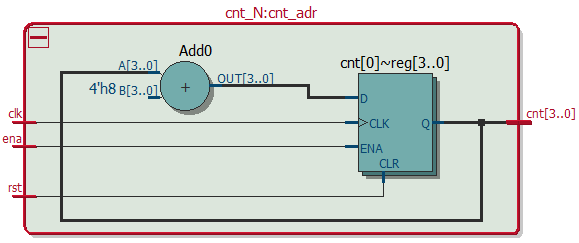
\includegraphics[width=0.7\textwidth]{elab7_1_rtl_2}
	\caption{Результат синтеза \code{cnt_adr} в RLT Viewer}
	\label{fig:elab7_1_rtl_2}
\end{center}
\end{figure}

\begin{figure}[H]
\begin{center}
	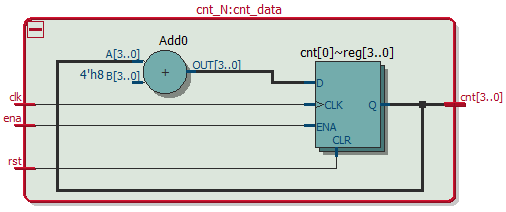
\includegraphics[width=0.7\textwidth]{elab7_1_rtl_3}
	\caption{Результат синтеза \code{cnt_data} в RLT Viewer}
	\label{fig:elab7_1_rtl_3}
\end{center}
\end{figure}

\subsection{Результаты моделирования}
\label{sec:elab7_1_modeling}

На рис. \ref{fig:elab7_1_modeling_1} -- \ref{fig:elab7_1_modeling} изображены временные диаграммы работы каждого модуля по отдельности и всего синтезированного устройства при \code{DIV = 3},\\ \code{N = 4}, \code{word_num = 16}, \code{data_W = 4}, \code{INV = 0}.

\begin{figure}[H]
\begin{center}
	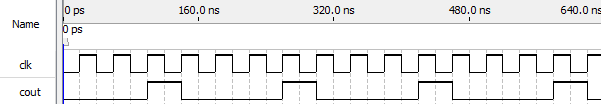
\includegraphics[width=\textwidth]{elab7_1_modeling_1}
	\caption{Результаты моделирования модуля \code{cnt_d}}
	\label{fig:elab7_1_modeling_1}
\end{center}
\end{figure}

\begin{figure}[H]
\begin{center}
	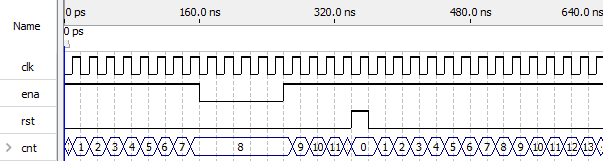
\includegraphics[width=\textwidth]{elab7_1_modeling_2}
	\caption{Результаты моделирования модуля \code{cnt_N}}
	\label{fig:elab7_1_modeling_2}
\end{center}
\end{figure}

\begin{figure}[H]
\begin{center}
	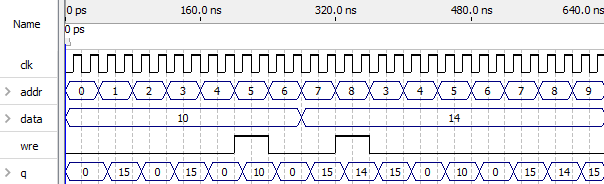
\includegraphics[width=\textwidth]{elab7_1_modeling_3}
	\caption{Результаты моделирования модуля \code{RAM}}
	\label{fig:elab7_1_modeling_3}
\end{center}
\end{figure}

\begin{figure}[H]
\begin{center}
	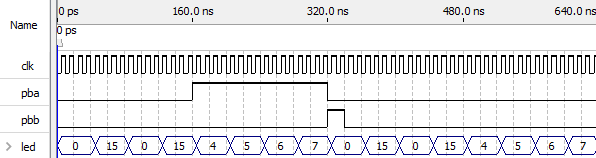
\includegraphics[width=\textwidth]{elab7_1_modeling}
	\caption{Результаты моделирования устройства}
	\label{fig:elab7_1_modeling}
\end{center}
\end{figure}

При моделировании устройства при активном уровне \code{pba} происходит запись в память, а при активном уровне \code{pbb} происходит асинхронный сброс. Сначала происходит чтение начальных данных, затем запись в память, после чего происходит асинхронный сброс и чтение записанных ранее данных.

\subsection{Назначение выводов СБИС}

На рис. \ref{fig:elab7_1_pins} приведены назначения выводов СБИС в Pin Planner.

\begin{figure}[H]
\begin{center}
	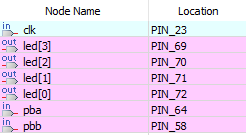
\includegraphics{elab7_1_pins}
	\caption{Таблица назначений в Pin Planer}
	\label{fig:elab7_1_pins}
\end{center}
\end{figure}

\subsection{Результаты проверки на плате}

Для тестирования проекта на плате были использованы тесты, описанные в пункте \ref{sec:elab7_1_modeling} при параметрах \code{DIV = 25_000_000}, \code{N = 4}, \code{word_num = 16}, \code{data_W = 4}, \code{INV = 1}. Результаты тестирования совпадают с ожидаемыми, следовательно, устройство работает верно.

\subsection{Выводы}

Реализовано описание параметризированного устройства, включающего счетчик-делитель, формирователи данных и адреса, модуль памяти и двоичный счетчик на сложение. Результаты моделирования и тестирования на плате показали, что разработанное устройство работает верно.

\section*{Заключение}

\addcontentsline{toc}{section}{\protect\numberline{}Заключение}

В данной работе рассмотрены основные принципы построения типовых устройств на языке описания аппаратуры Verilog, таких как: 
\begin{itemize}
	\item одноразрядный полусумматор и полный одноразрядный сумматор;
	\item полный сумматор с последовательным переносом;
	\item беззнаковый делитель с точностью 4 знака после запятой;
	\item знаковый умножитель на фиксированное число;
	\item преобразователь двоичного кода в код Грея;
	\item преобразователь кода Грея в двоичный код;
	\item реверсивный счетчик с динамически изменяемым модулем счета;
	\item параметризированное АЛУ;
	\item конечный автомат на основе счетчика;
	\item N-разрядный последовательный умножитель;
	\item параметризированное устройство с модулем памяти. 
\end{itemize}

Рассмотрены основные конструкции языка Verilog и получены практические навыки проектирования устройств с помощью Verilog, их моделирования, тестирования на физической модели и отладки.

\end{document}